\documentclass[10pt]{article}
\usepackage{graphicx}
\usepackage{geometry}
\usepackage{url}
\geometry{
 a4paper,
 total={220mm,297mm},
 left=10mm,
 right=20mm,
 top=20mm,
 bottom=20mm,
 }
\begin{document}
\begin{flushright}
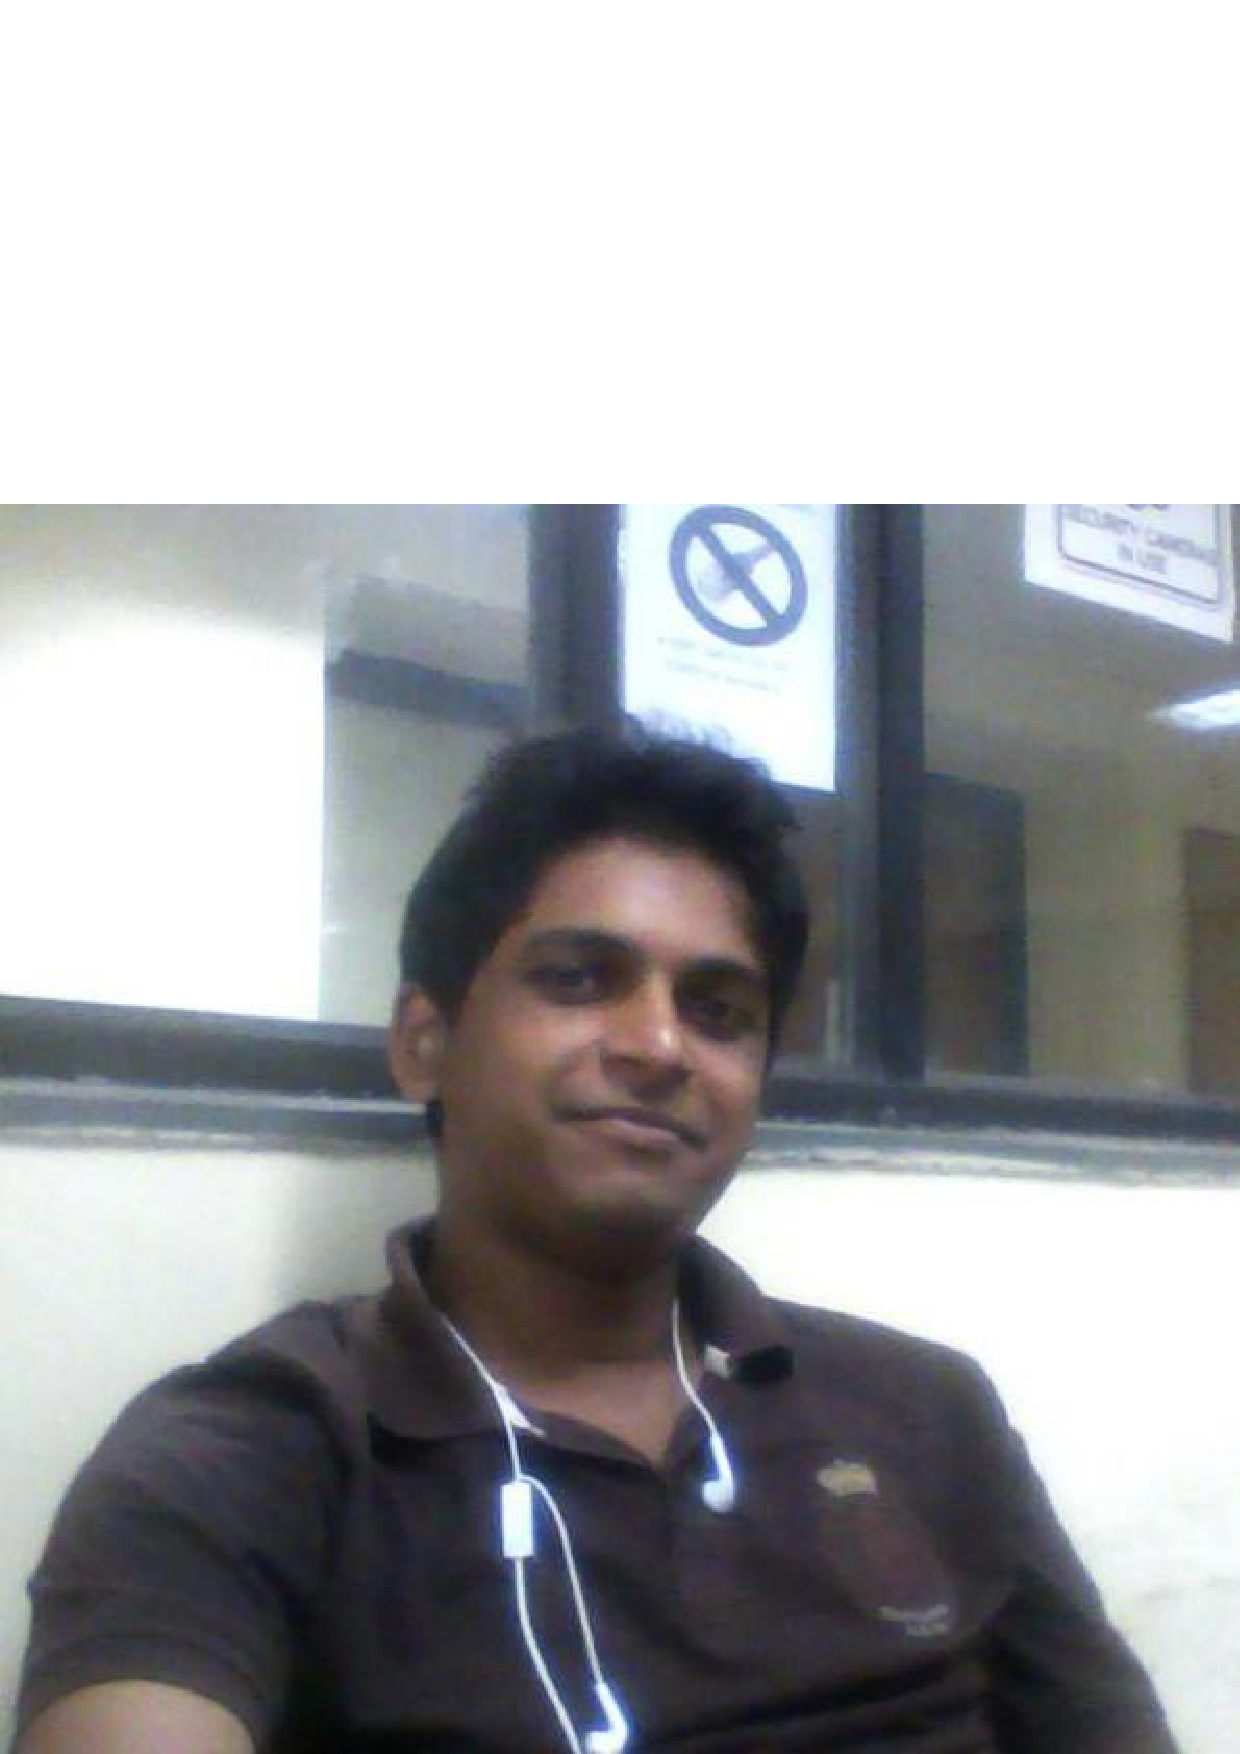
\includegraphics[scale=0.25,bb=0 0 300 300]{myimage.jpg}
\end{flushright}
\begin{flushleft}
{\huge \textbf{AMIT KUMAR}}\\
Second Year Undergraduate \hspace{85mm}
 Phone: 9795309466\\
Department of Computer Science\\
Roll no - 13094\\
Website :\url{home.iitk.ac.in}\\
Email id:\url{kmramit@iitk.ac.in}\\
\end{flushleft}
\begin{flushleft}
\begin{center}
{\large \textbf{TRANSCRIPT} }
\end{center}
\begin{tabular}{c c c c c c c}
\hline 
YEAR/SEM & COURSE NO & TITLE & UNIT & GRADE & SPI & CPI\\
\hline
2013-2014 FIRST & CHM101 & CHEMISTRY LABORATORY & 3 & A\\
  & ESC101A & {\small  FUNDAMENTAL OF COMPUTING} & 14 & A\\
  & MTH101A &  MATHEMATICS I & 11 & A\\
 & PE101A & MORNING EXERCISE & 3 & S\\
  & PHY103A & PHYSICS-II & 11 & A\\
  & SOC171A & INTRODUCTORY SOCIOLOGY & 11 & A\\
 & & & & & 10.0 & 10.0\\ 
 & & & & & &\\
 2013-14 SECOND & CHM102A  & GENERAL CHEMISTRY & 8 & B\\
   & LIF101A & INTRODUCTION TO BIOLOGY & 6 & A\\
   & MTH102A  & MATHEMATICS -II & 11 & A\\
   & PE102A & EVENING EXERCISE & 3 & S\\
   &PHY101A &  PHYSICS LABORATORY & 3 & A*\\
   &PHY102A & PHYSICS - I & 11 & B\\
   &TA101A& ENGINEERING GRAPHICS & 9 & A\\
   & & & & & 9.2 & 9.6 \\
   & & & & & & \\
2014-15 THIRD & COM200 & COMMUNICATION SKILLS: COMPOSITION & 5 & S\\
  & CS201A & MATHEMATICS FOR COMPUTER SCIENCE -I & 9 & B\\
  & CS210A &  DATA SRTUCTURE AND ALGORITHMS & 12 & B\\
  & ESC201A & INTRODUCTION TO ELECTRONICS & 14 & A \\
  & ESO204A & FLUID MECHANICS AND RATE PROCESSES & 11 & B\\
  & TA201A & MANUFACTURING PROCESSES -I & 6 & B\\
  & & & & & 8.5 & 9.2\\
  & & & & & &\\
\end{tabular}
{\large \textbf{EDUCATIONAL QUALIFICATION}}
\begin{tabular}{c c c c}
\hline \hline
Year & Degree & School/Institution & CPI/Percentage\\
\hline
2013-present & B-Tech & Indian Institute of Technology Kanpur & 9.24\\
2013 & XII & The Avadh School & 96.0 \\
2011 & X & Nirmala Convent Inter College & 95.2\\
\hline \\
\end{tabular}
{\large \textbf{\underline{SCHOLISTIC ACHIEVEMENTS}}}
\begin{description}
\item[$\bullet$]Secured 60th rank in ACM ICPC Amritapuri Regionals among 1600 national teams
\item[$\bullet$]Secured All India Rank – 1128 in JEE Advanced among more than 0.5 million aspirants
\item[$\bullet$]Secured All India Rank – 421 in JEE Mains among more than 1.2 million aspirants
\item[$\bullet$]Secured AIR - 62 in Kishore Vaigyanik Protsahan Yojana (KVPY) -2012 out of 40,000 students
\item[$\bullet$]Secured AIR -76 in National Science Level Talent Search Examination (NSTSE) 2011
\item[$\bullet$]Qualified National Standard Examination in Physics (NSEP) 2012 among 300 students in India
\item[$\bullet$]Qualified National Standard Examination in Chemistry (NSEC) 2012 among 300 students in India
\item[$\bullet$]Awarded Best Staff Pick Project in Manufacturing processes course
\item[$\bullet$]School Topper in (X) ICSE 2011 and (XII)CBSE 2013  with 100\% marks in Environmental Education(ICSE)
\end{description}
{\large \textbf{\underline{PROJECTS}}}\\
\textbf{\underline{Programming Club Website Development}}
\begin{description}
\item[$\bullet$]Developed a fully login based website with the facility to upload tutorial, projects, documentation
\item[$\bullet$]Website has a forum for discussing various issues
\item[$\bullet$]Used iFrame to add google calendar for various PCLub(Programming Club) events
\item[$\bullet$]Used Web Scraping to automatically update CodeChef Ranking of Students of IIT Kanpur after every contest
\item[$\bullet$]Used Twitter APIs to get the latest updates of famous personalities and technology news\\
\end{description}
\textbf{\underline{Advanced Track Project Under Prof. Surendar Baswana}}
\begin{description}
\item[$\bullet$]Designed two algorithm (first one time efficient and other memory efficient) for a Geometric Data Structure Problem
\item[$\bullet$]Detailed Analysis and Proofs of Complexity of Time and Space for both he approach
\item[$\bullet$]Ran the program on data upto million numbers and made comparison between the two data structures\\
\end{description}
\textbf{\underline{Open Air Theatre(As a part of course TA201)	}}
\begin{description}
\item[$\bullet$]Manufactured a replica of Open Air Theartre, IIT Kanpur using various manufacturing processes like welding,casting,brazing and metal sheet forming.
\end{description}
{\large \textbf{\underline{TECHNICAL SKILLS}}}\\
\textbf{Programming Language}: C , C++, Python ,Java , Verilog\\
\textbf{Web Development}: HTML5, CSS, Ajax ,Jquery,PHP\\
\textbf{Platform}: Windows, Linux(Ubuntu , Fedora, Debian)\\
\textbf{Frameworks}: CodeIgniter, Semantic UI\\
\textbf{Software and Utilities}: Git, 3Ds max,Latex , Vim,Solidworks\\
\textbf{Database Systems}: MySql\\
{\large \textbf{\underline{RELEVANT COURSES UNDERTAKEN}}}\\
\begin{tabular}{c c c c}
\hline \hline
ESC101 & Fundamental of computing & ESC201 & Introduction of Electronics\\
CS210 & Data structures and Algorithms & TA101 & Engineering Graphics\\
CS201 & Discrete Mathematics & TA201 & Manufacturing processes\\
CS220 & Computer Organization and Architecture & CS202 & Logic in Computer Science \\
\hline \\
\end{tabular}
{\large \textbf{\underline{POSITIONS OF RESPONSIBILITY}}}\\
\textbf{Student Guide} under the Counselling Service, IIT Kanpur
\begin{description}
\item[$\bullet$]Mentored 6 freshmen,guided and supported them academically and emotionally during their  initial  period of stay at  IIT Kanpur and  was also responsible for their smooth and comfortable transi- -tion to college environment
\end{description}
{\large \textbf{\underline{EXTRA-CURRICULAR ACTIVITIES AND ACHIEVEMENTS}}}
\begin{description}
\item[$\bullet$]Active user in various Programming websites like CodeChef and SPOJ
\item[$\bullet$]Stood 3rd in 24 hours Freshers Programming Contest
\item[$\bullet$]Secured 70th position in ACM ICPC Gwalior Online Round 2014
\item[$\bullet$]Participated in various Card Games (Poker, 29) held in IIT Kanpur
\item[$\bullet$]Play Volley Ball, Badminton, Table Tennis and Basketball. Had Volley Ball as CPA (Compulsory Physical Activities)
\item[$\bullet$]Participated in District Athletics Meet in 100m Sprint and Hurdle race
\end{description}
\end{flushleft}
\end{document}
